\documentclass{standalone}
\usepackage{amsmath}
\usepackage{tikz}

\begin{document}

\begin{tikzpicture}[scale=1,baseline={(0,0)}]
\draw [black, line width=0.6pt, ->] (0,0) to[out=90,in=270] (0,4.25);
\node [anchor=south] at (0,4.5) {y};
\draw [black, line width=0.6pt, ->] (-4.25,0) to[out=0,in=180] (4.25,0);
\node [anchor=west] at (4.5,0) {x};

\draw [blue, line width=0.6pt] (-4.25,4.0) to[out=0,in=180] (4.25,4.0);
\draw [blue, line width=0.6pt] (-4.25,2.0) to[out=0,in=180] (4.25,2.0);
\draw [green, line width=0.6pt] (-3.5,0) to[out=90,in=270] (-3.5,4.5);

\node[anchor=45] at (0.0,4.0) {$O$};
\node[anchor=45] at (-3.5,4.0) {$Q$};
\node[anchor=45] at (-3.5,2.0) {$P$};
\node[anchor=225] at (-2.0,4.1) {$x = u$};
\node[anchor=225] at (-3.0,1.0) {$y = e^v$};

\end{tikzpicture}

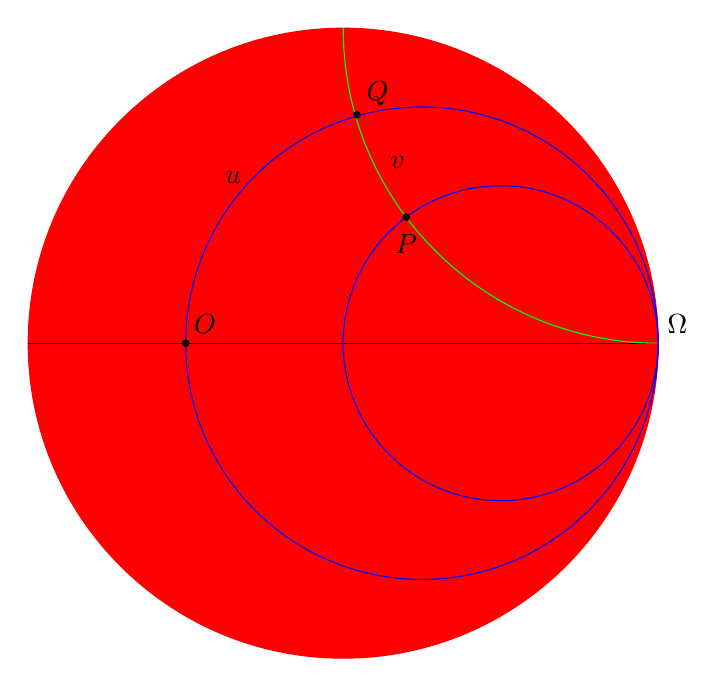
\begin{tikzpicture}[scale=1,baseline={(0,0)}]
    \node[anchor=225] at (4,2) {$\Omega$};
    \draw[red,fill=red] (0,2) circle[radius=4];
    \draw[blue] (1, 2) circle[radius=3];
    \draw[black] (-4,2) -- (4,2);
    \draw[green] (4,2) arc (-90:-180:4);
    \draw[blue] (2, 2) circle[radius=2];
    \node[fill,circle,inner sep=1pt] at (-2,2) {};
    \node[anchor=225] at (-2,2) {$O$};
    \node[fill,circle,inner sep=1pt] at (0.175,4.9) {};
    \node[anchor=225] at (0.175,4.9) {$Q$};
    \node[fill,circle,inner sep=1pt] at (0.8,3.6) {};
    \node[anchor=90] at (0.8,3.5) {$P$};
    \node[anchor=225] at (0.49,4.1) {$v$};
    \node[anchor=225] at (-1.6,3.9) {$u$};
\end{tikzpicture}
\end{document}
